\documentclass{article}
\usepackage{spikey}
\usepackage{amsmath}
\usepackage{mathrsfs}
\usepackage{amssymb}
\usepackage{soul}
\usepackage{float}
\usepackage{graphicx}
\usepackage{hyperref}
\usepackage{fancyhdr}
%\usepackage{xcolor}
\usepackage{chngcntr}
\usepackage{centernot}
\usepackage[shortlabels]{enumitem}
\usepackage[margin=1truein]{geometry}
\usepackage{tkz-graph}
\usepackage{dsfont}
\usepackage{caption}
\usepackage{subcaption}
\usepackage{booktabs}
\usepackage[yyyymmdd,hhmmss]{datetime}

\usepackage{tikz}
\usetikzlibrary{arrows}

\usepackage{setspace}
\linespread{1.15}
\usepackage[margin=1truein]{geometry}

\counterwithin{equation}{section}
\counterwithin{figure}{section}

\usepackage{listings}
 
\definecolor{codegreen}{rgb}{0,0.6,0}
\definecolor{codegray}{rgb}{0.5,0.5,0.5}
\definecolor{codeblue}{rgb}{0.3,0.5,0.8}
\definecolor{codepurple}{rgb}{0.58,0,0.82}
%\definecolor{backcolour}{rgb}{0.95,0.95,0.92}
\definecolor{backcolour}{rgb}{1,1,1}

\lstdefinestyle{mystyle}{
    backgroundcolor=\color{backcolour},   
    commentstyle=\color{codegreen},
    keywordstyle=\color{magenta},
    numberstyle=\tiny\color{codegray},
    stringstyle=\color{codepurple},
    basicstyle=\ttfamily\footnotesize,
    breakatwhitespace=false,         
    breaklines=true,                 
    captionpos=b,                    
    keepspaces=true,                 
    numbers=left,                    
    numbersep=5pt,                  
    showspaces=false,                
    showstringspaces=false,
    showtabs=false,                  
    tabsize=4
}

\lstset{style=mystyle}

\title{CSC413: Programming Assignment 4}
\date{\today\ at \currenttime}
\author{Tianyu Du (1003801647)}
\begin{document}
	\maketitle
	\section{Part 1: Deep Convolutional GAN (DCGAN) [4pt]}
	\subsection{Generator}
	\textbf{Implementation} Note that I reshaped the input in \texttt{forward} method as well.
	\begin{lstlisting}[language=python]
class DCGenerator(nn.Module):
    def __init__(self, noise_size, conv_dim, spectral_norm=False):
        super(DCGenerator, self).__init__()

        self.conv_dim = conv_dim # 32

        ###########################################
        ##   FILL THIS IN: CREATE ARCHITECTURE   ##
        ###########################################
        self.linear_bn = nn.Sequential(
            nn.Linear(noise_size, self.conv_dim*4*4*4),
            nn.BatchNorm1d(self.conv_dim*4*4*4)
        ) # (100, 2048)
        self.upconv1 = upconv(self.conv_dim*4, self.conv_dim*2, 5, stride=2, padding=2, batch_norm=True, spectral_norm=spectral_norm)
        self.upconv2 = upconv(self.conv_dim*2, self.conv_dim, 5, stride=2, padding=2, batch_norm=True, spectral_norm=spectral_norm)
        self.upconv3 = upconv(self.conv_dim, 3, 5, stride=2, padding=2, batch_norm=False, spectral_norm=spectral_norm)

    def forward(self, z):
        """
        ...
        """
        batch_size = z.size(0)
        ###########################################
        ##   		RESHAPED HERE AS WELL	     ##
        ###########################################
        z = z.view(batch_size, -1)
        out = F.relu(self.linear_bn(z)).view(-1, self.conv_dim*4, 4, 4)    # BS x 128 x 4 x 4
        out = F.relu(self.upconv1(out))  # BS x 64 x 8 x 8
        out = F.relu(self.upconv2(out))  # BS x 32 x 16 x 16
        out = F.tanh(self.upconv3(out))  # BS x 3 x 32 x 32
        
        out_size = out.size()
        if out_size != torch.Size([batch_size, 3, 32, 32]):
            raise ValueError("expect {} x 3 x 32 x 32, but get {}".format(batch_size, out_size))
        return out
	\end{lstlisting}

	\subsection{Training Loop}
	\textbf{Implementation}
	\begin{lstlisting}[language=python]
def gan_training_loop(dataloader, test_dataloader, opts):
    ...

            for d_i in range(opts.d_train_iters):
                d_optimizer.zero_grad()

                # FILL THIS IN
                # 1. Compute the discriminator loss on real images
                D_real_loss = torch.mean((D(real_images) - 1) ** 2) / 2

                # 2. Sample noise
                noise = sample_noise(real_images.shape[0], opts.noise_size)

                # 3. Generate fake images from the noise
                fake_images = G(noise)
                
                # 4. Compute the discriminator loss on the fake images
                D_fake_loss = torch.mean(D(fake_images) ** 2) / 2

                # ---- Gradient Penalty ----
                if opts.gradient_penalty:
                    ...
                else:
                    gp = 0.0

                # --------------------------
                # 5. Compute the total discriminator loss
                D_total_loss = D_real_loss + D_fake_loss + gp

                D_total_loss.backward()
                d_optimizer.step()

            ###########################################
            ###          TRAIN THE GENERATOR        ###
            ###########################################

            g_optimizer.zero_grad()

            # FILL THIS IN
            # 1. Sample noise
            noise = sample_noise(real_images.shape[0], opts.noise_size)

            # 2. Generate fake images from the noise
            fake_images = G(noise)

            # 3. Compute the generator loss
            G_loss = torch.mean((D(fake_images) - 1)**2)

            G_loss.backward()
            g_optimizer.step()
            ...
	\end{lstlisting}
	\subsection{Experiments}
	\paragraph{Experiment 1} These two figures below shows the generated results at 1,000 iterations and 20,000 iterations without gradient penalty. The generated results at 20,000 are much more shaper (i.e., with clearer boundaries) than 1,000 iteration results, but colours of generated samples after 20,000 iterations are darker.
	\begin{figure}[H]
		\centering
		\caption{1,000 iters (left) and 20,000 iters (right)}
		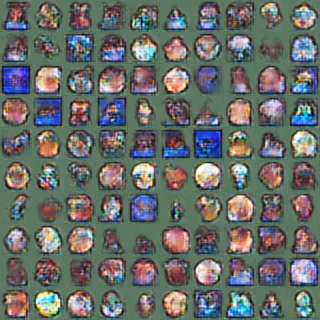
\includegraphics[width=0.45\linewidth]{./samples_dcgan_normal/sample-001000.png}
		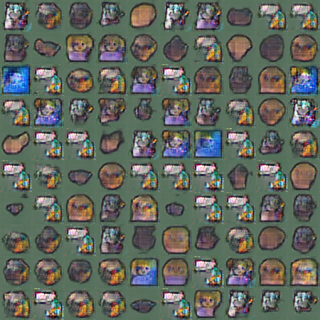
\includegraphics[width=0.45\linewidth]{./samples_dcgan_normal/sample-020000.png}
		\label{Q1:wo}
	\end{figure}

	\paragraph{Experiment 2} Two figures below are generated samples from a GAN with gradient penalty after being trained for 1,000 iterations and 20,000 iterations. Compared samples in figure \ref{Q1:wo}, these samples are now with even clearer boundaries, and colours are more vivid. The gradient penalty term added prevent gradient exploding while training the discriminator, and helps stabilize the training. So that adding gradient penalty improve generalizability of the model.  
	\begin{figure}[H]
		\centering
		\caption{1,000 iters (left) and 20,000 iters (right)}
		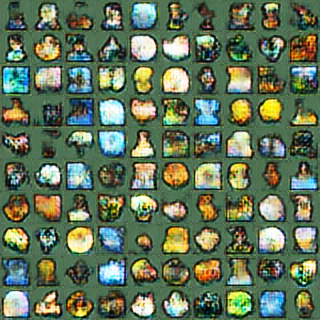
\includegraphics[width=0.45\linewidth]{./samples_dcgan_gp_alpha_alpha/sample-001000.png}
		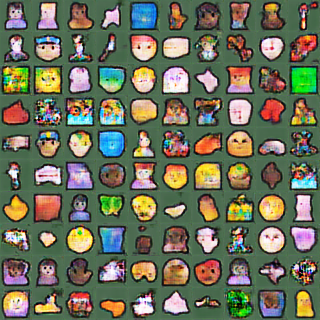
\includegraphics[width=0.45\linewidth]{./samples_dcgan_gp_alpha_alpha/sample-020000.png}
	\end{figure}
	
	\section{Part 2: CycleGAN [3pt]}
	\subsection{CycleGAN Experiments}
	\subsubsection{Question 1}
	\paragraph{Answer} Default configurations at 200 iterations: 
	\begin{figure}[H]
		\centering
		\caption{Iteration 200, left: $X \to Y$, right: $Y \to X$}
		
\includegraphics[width=0.45\linewidth]{./samples_cyclegan_Q1/sample-000200-X-Y.png}
		
\includegraphics[width=0.45\linewidth]{./samples_cyclegan_Q1/sample-000200-Y-X.png}
	\end{figure}
	\begin{figure}[H]
		\centering
		\caption{Iteration 5000, left: $X \to Y$, right: $Y \to X$}
		
\includegraphics[width=0.45\linewidth]{./samples_cyclegan_Q1/sample-005000-X-Y.png}
		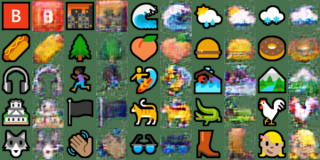
\includegraphics[width=0.45\linewidth]{./samples_cyclegan_Q1/sample-005000-Y-X.png}
	\end{figure}

	\subsubsection{Question 2}
	\paragraph{Answer} Changed the random seed to \texttt{SEED = 42} (originally 4). With the new random seed, some images in the final $Y \to X$ translations are more clear and with less background noise. Such as boot (row 5, item 4), mountain (row 3, item 5), and donut (row 2, item 5).
	\todo{Explain differences}
	\begin{figure}[H]
		\centering
		\caption{Iteration 200, left: $X \to Y$, right: $Y \to X$}
		
\includegraphics[width=0.45\linewidth]{./samples_cyclegan_Q2_seed42/sample-000200-X-Y.png}
		
\includegraphics[width=0.45\linewidth]{./samples_cyclegan_Q2_seed42/sample-000200-Y-X.png}
	\end{figure}
	\begin{figure}[H]
		\centering
		\caption{Iteration 5000, left: $X \to Y$, right: $Y \to X$}
		
\includegraphics[width=0.45\linewidth]{./samples_cyclegan_Q2_seed42/sample-005000-X-Y.png}
		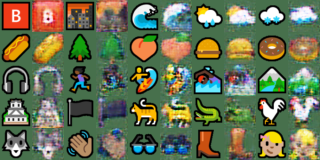
\includegraphics[width=0.45\linewidth]{./samples_cyclegan_Q2_seed42/sample-005000-Y-X.png}
	\end{figure}

	\subsubsection{Question 3}
	\todo{Add comment}
	\paragraph{Comments} I tried three different level of lambda values for the cycle consistency, translation results are attached below:
	\paragraph{Configuration 1} \texttt{lambda\_cycle = 0}, all other hyper-parameters are default, including the random seed.
	\begin{figure}[H]
		\centering
		\caption{ \texttt{lambda\_cycle = 0}, iteration 200, left: $X \to Y$, right: $Y \to X$}
		
\includegraphics[width=0.45\linewidth]{./samples_cyclegan_Q3_lambda0/sample-000200-X-Y.png}
		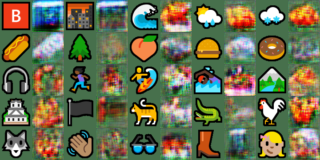
\includegraphics[width=0.45\linewidth]{./samples_cyclegan_Q3_lambda0/sample-000200-Y-X.png}
	\end{figure}
	\begin{figure}[H]
		\centering
		\caption{ \texttt{lambda\_cycle = 0}, iteration 5000, left: $X \to Y$, right: $Y \to X$}
		
\includegraphics[width=0.45\linewidth]{./samples_cyclegan_Q3_lambda0/sample-005000-X-Y.png}
		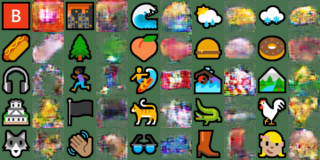
\includegraphics[width=0.45\linewidth]{./samples_cyclegan_Q3_lambda0/sample-005000-Y-X.png}
	\end{figure}

	\paragraph{Configuration 2} \texttt{lambda\_cycle = 0.03}, all other hyper-parameters are default, including the random seed.
	\begin{figure}[H]
		\centering
		\caption{ \texttt{lambda\_cycle = 0.03}, iteration 200, left: $X \to Y$, right: $Y \to X$}
		
\includegraphics[width=0.45\linewidth]{./samples_cyclegan_Q3_lambda0_03/sample-000200-X-Y.png}
		
\includegraphics[width=0.45\linewidth]{./samples_cyclegan_Q3_lambda0_03/sample-000200-Y-X.png}
	\end{figure}
	\begin{figure}[H]
		\centering
		\caption{ \texttt{lambda\_cycle = 0.03}, iteration 5000, left: $X \to Y$, right: $Y \to X$}
		
\includegraphics[width=0.45\linewidth]{./samples_cyclegan_Q3_lambda0_03/sample-005000-X-Y.png}
		
\includegraphics[width=0.45\linewidth]{./samples_cyclegan_Q3_lambda0_03/sample-005000-Y-X.png}
	\end{figure}

	\paragraph{Configuration 3} \texttt{lambda\_cycle = 0.3}, all other hyper-parameters are default, including the random seed.
	\begin{figure}[H]
		\centering
		\caption{ \texttt{lambda\_cycle = 0.3}, iteration 200, left: $X \to Y$, right: $Y \to X$}
		
\includegraphics[width=0.45\linewidth]{./samples_cyclegan_Q3_lambda0_3/sample-000200-X-Y.png}
		
\includegraphics[width=0.45\linewidth]{./samples_cyclegan_Q3_lambda0_3/sample-000200-Y-X.png}
	\end{figure}
	\begin{figure}[H]
		\centering
		\caption{ \texttt{lambda\_cycle = 0.3}, iteration 5000, left: $X \to Y$, right: $Y \to X$}
		
\includegraphics[width=0.45\linewidth]{./samples_cyclegan_Q3_lambda0_3/sample-005000-X-Y.png}
		
\includegraphics[width=0.45\linewidth]{./samples_cyclegan_Q3_lambda0_3/sample-005000-Y-X.png}
	\end{figure}

	\paragraph{Configuration 4} \texttt{lambda\_cycle = 1.0}, all other hyper-parameters are default, including the random seed.
	\begin{figure}[H]
		\centering
		\caption{ \texttt{lambda\_cycle = 1.0}, iteration 200, left: $X \to Y$, right: $Y \to X$}
		
\includegraphics[width=0.45\linewidth]{./samples_cyclegan_Q3_lambda1/sample-000200-X-Y.png}
		
\includegraphics[width=0.45\linewidth]{./samples_cyclegan_Q3_lambda1/sample-000200-Y-X.png}
	\end{figure}
	\begin{figure}[H]t
		\centering
		\caption{ \texttt{lambda\_cycle = 1.0}, iteration 5000, left: $X \to Y$, right: $Y \to X$}
		
\includegraphics[width=0.45\linewidth]{./samples_cyclegan_Q3_lambda1/sample-005000-X-Y.png}
		
\includegraphics[width=0.45\linewidth]{./samples_cyclegan_Q3_lambda1/sample-005000-Y-X.png}
	\end{figure}

	\section{Part 3: BigGAN [2pt]}
	\subsection{BigGAN Experiments}
	\subsubsection{Question 1}
	\paragraph{Method} Given two classes with embeddings $\mathbf{r}_{class1}$ and $\mathbf{r}_{class2}$ in T-SNE space, to decide whether they are good candidate for linear interpolation, I looked at convex combinations of two classes' embeddings in figure \ref{tsne}.
	Let $\Phi$ denote the set of convex combinations:
	\begin{align}
		\Phi = \{\alpha \mathbf{r}_{c l a s s 1}+(1-\alpha) \mathbf{r}_{c l a s s 2}: \alpha \in[0,1]\}
	\end{align}
	Linear interpolations between these two classes are basically taking points in set $\Phi$ and visualizing them.
	If there are many \ul{other classes' embeddings} on or near the set $\Phi$, points in $\Phi$ are likely to be associated with meaningful visualizations.
	Therefore, linear interpolations between these two classes are likely to generate meaningful results.
	Otherwise, these two classes are not good candidates for linear interpolation.
	\begin{figure}[H]
		\caption{T-SNE Plot}
		\centering
		\label{tsne}
		\medbreak
		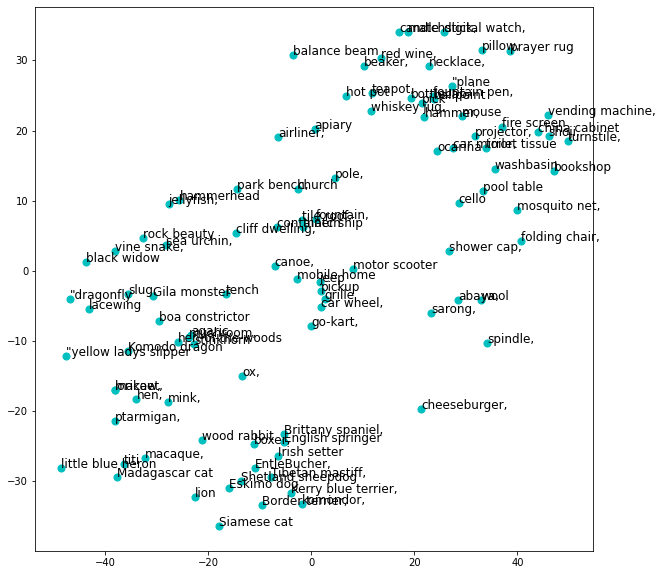
\includegraphics[width=0.7\linewidth]{./tsne.png}
	\end{figure}
	\paragraph{Good Candidate Match 1} There are many classes near the segment between \texttt{folding chair} and \texttt{vending machine} (right-up corner), so linear interpolation should be meaningful.
%	\begin{figure}[H]
%		\caption{Folding Chair and Vending Machine}
%		\centering
%		\medbreak
%		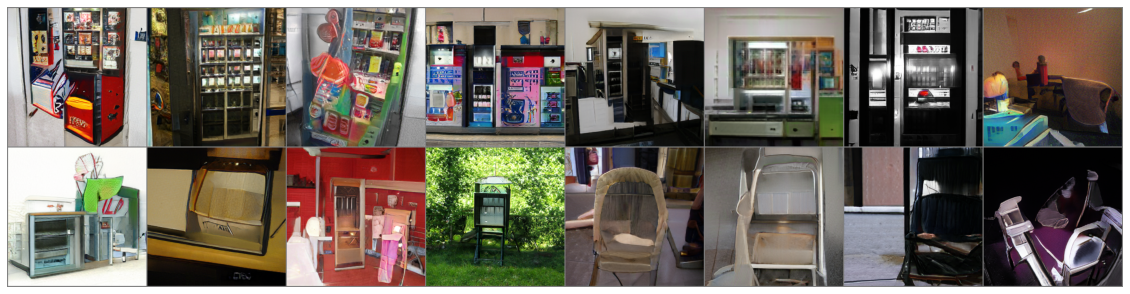
\includegraphics[width=0.7\linewidth]{./foldingchair_vendingmachine.png}
%	\end{figure}
	
	\paragraph{Good Candidate Match 2} Similarly, there are many classes on the line between \texttt{bookshop} and \texttt{hot pot} (right-up corner), so they are ideal for linear interpolation.

%	\begin{figure}[H]
%		\caption{Hot Pot and Bookshop}
%		\centering
%		\medbreak
%		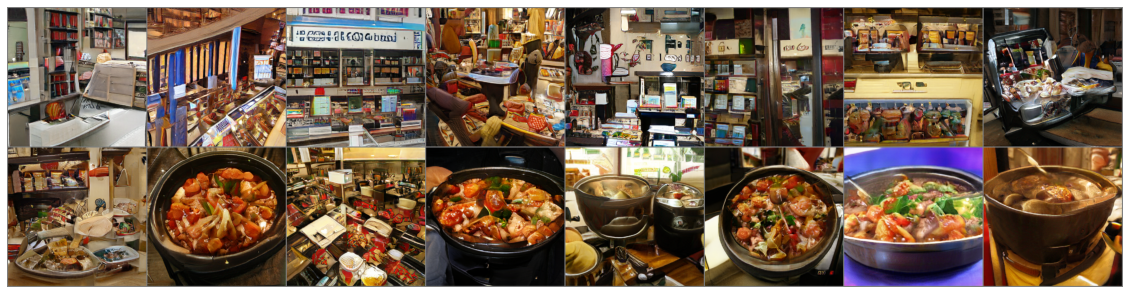
\includegraphics[width=0.7\linewidth]{./hotpot_bookshop.png}
%	\end{figure}
	
	\paragraph{Bad Candidate Match 1} There are no other classes' embeddings are in between embeddings of \texttt{Go-Kart} and \texttt{Chessburger} in T-SNE plot, so they are not good match.
%	\begin{figure}[H]
%		\caption{Go-Kart and Chessburger}
%		\centering
%		\medbreak
%		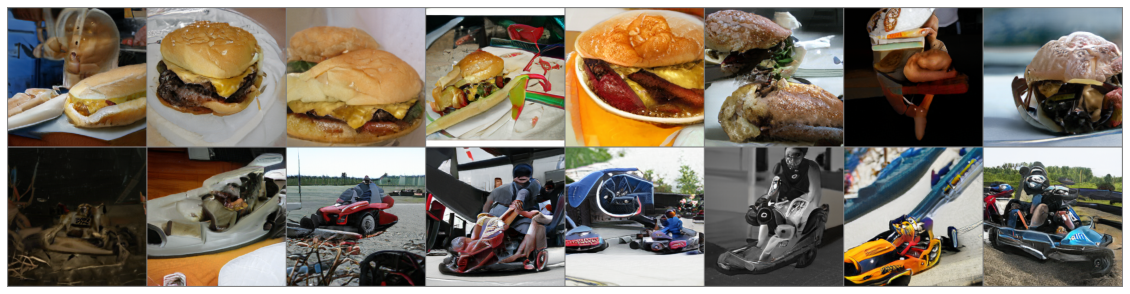
\includegraphics[width=0.7\linewidth]{./gokart_cheeseburger.png}
%	\end{figure}

	\paragraph{Bad Candidate Pair 2} Similarly, \texttt{Ox} and \texttt{Chessburger} are not good match.
%	\begin{figure}[H]
%		\caption{Ox and Chessburger}
%		\centering
%		\medbreak
%		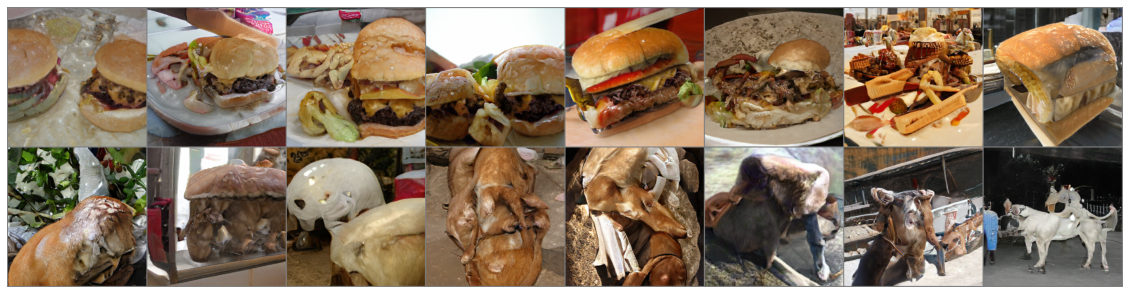
\includegraphics[width=0.7\linewidth]{./ox_chessburger.png}
%	\end{figure}

	\subsubsection{Question 2}
	\textbf{Implementation}
	\begin{lstlisting}[language=python]
#Linear interpolation between two class embedings
def generate_linear_interpolate_sample(G, batch_size, class_label1, class_label2, alpha):
  	G.eval()
  	G.to(DEVICE)
  	with torch.no_grad():
	    z = torch.randn(batch_size, G.dim_z).to(DEVICE)
	    class1_emb = G.shared(torch.tensor(class_label1).to(DEVICE)*torch.ones((batch_size,)).to(DEVICE).long())
	    class2_emb = G.shared(torch.tensor(class_label2).to(DEVICE)*torch.ones((batch_size,)).to(DEVICE).long())
	
	    ###########################################
	    ##   FILL THIS IN: CREATE NEW EMBEDDING  ##
	    ###########################################    
	    new_emb = alpha * class1_emb + (1 - alpha) * class2_emb
	
	    images = G(z, new_emb)
  	return images
	\end{lstlisting}
	\textbf{Linear Interpolation Results}
	\begin{figure}[H]
		\caption{Good Match 1: Folding Chair and Vending Machine}
		\centering
		\medbreak
		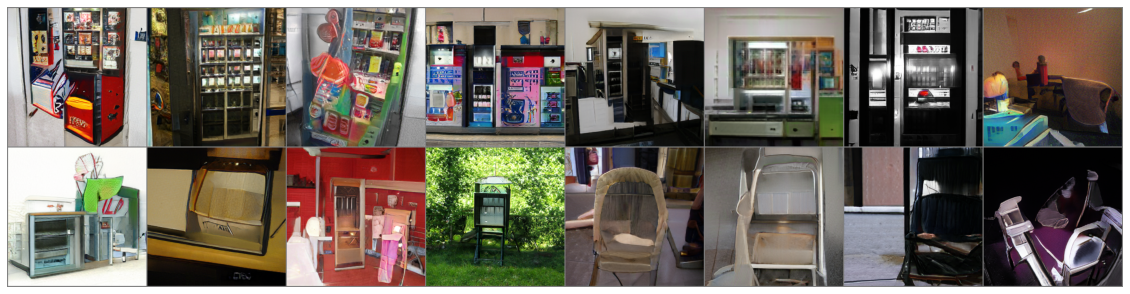
\includegraphics[width=0.7\linewidth]{./foldingchair_vendingmachine.png}
	\end{figure}

	\begin{figure}[H]
		\caption{Good Match 2 Hot Pot and Bookshop}
		\centering
		\medbreak
		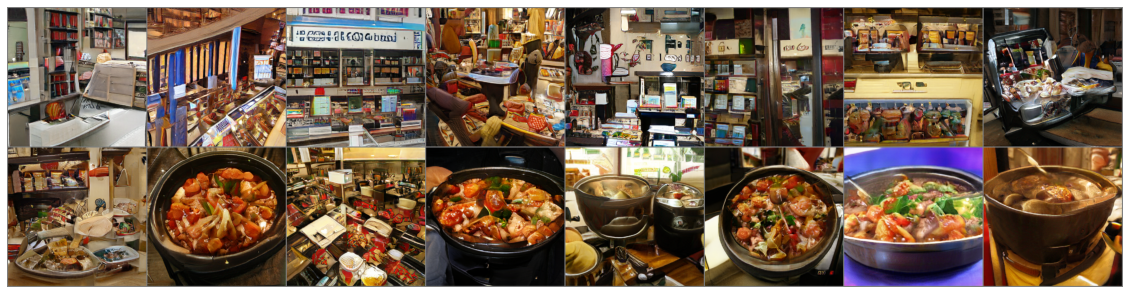
\includegraphics[width=0.7\linewidth]{./hotpot_bookshop.png}
	\end{figure}
	
	\begin{figure}[H]
		\caption{Bad Match 1 Go-Kart and Chessburger}
		\centering
		\medbreak
		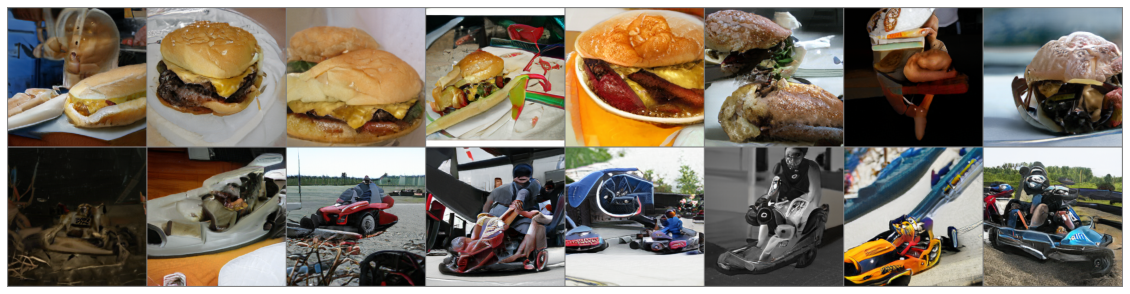
\includegraphics[width=0.7\linewidth]{./gokart_cheeseburger.png}
	\end{figure}

	\begin{figure}[H]
		\caption{Bad Match 2 Ox and Chessburger}
		\centering
		\medbreak
		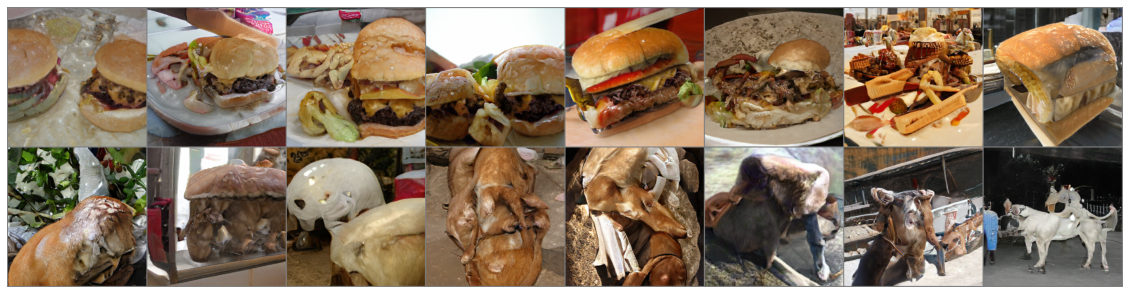
\includegraphics[width=0.7\linewidth]{./ox_chessburger.png}
	\end{figure}
\end{document}

































